% The three damage levels, with the empty one drawn empty.
% No generator: this is the taxonomy of Section 3.3, not a measurement. Only the level
% assignment the text states explicitly (ROAD supports L1; L3 is not identified) appears here; can-train-and-test
% is deliberately absent because the paper never assigns it a level, and inferring one from
% its rho_< would be the figure making a claim the manuscript does not.
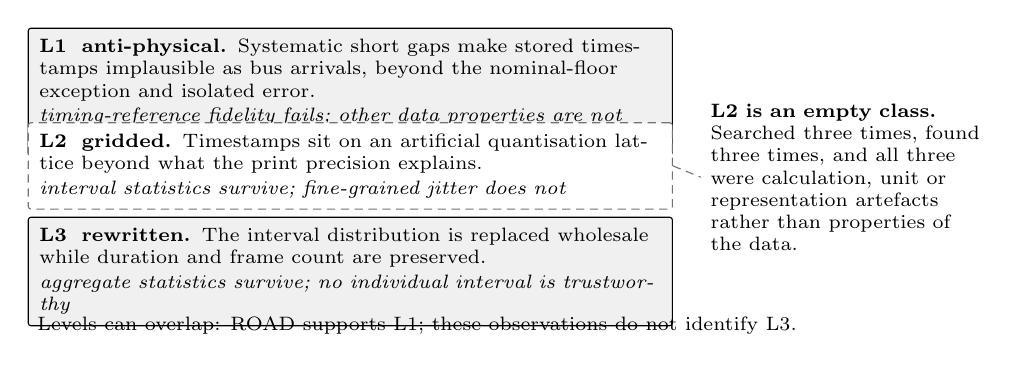
\begin{tikzpicture}[font=\scriptsize, x=1cm, y=1cm]
\tikzset{
  lvl/.style={draw, rounded corners=1pt, minimum height=1.02cm, text width=7.9cm,
              inner sep=4pt, align=left, anchor=north west},
  full/.style={lvl, fill=black!6},
  hollow/.style={lvl, fill=white, densely dashed, draw=black!55},
  tag/.style={font=\fontsize{6.6}{7.4}\selectfont, anchor=north west, inner sep=0pt},
}

\node[full] at (0,0)
  {\textbf{L1 \ anti-physical.} Systematic short gaps make stored timestamps
   implausible as bus arrivals, beyond the nominal-floor exception and isolated error.\\[1pt]
   \textit{\fontsize{6.6}{7.4}\selectfont timing-reference fidelity fails; other data properties are not assessed}};

\node[hollow] (l2box) at (0,-1.20)
  {\textbf{L2 \ gridded.} Timestamps sit on an artificial quantisation lattice beyond
   what the print precision explains.\\[1pt]
   \textit{\fontsize{6.6}{7.4}\selectfont interval statistics survive; fine-grained jitter does not}};

\node[full] at (0,-2.40)
  {\textbf{L3 \ rewritten.} The interval distribution is replaced wholesale while duration
   and frame count are preserved.\\[1pt]
   \textit{\fontsize{6.6}{7.4}\selectfont aggregate statistics survive; no individual interval is trustworthy}};

% The empty class is the result, so it is marked on the figure rather than left to the text.
\node[anchor=west, font=\scriptsize, align=left, text width=3.5cm] (l2note)
     at (8.55,-1.90)
     {\textbf{L2 is an empty class.}\\ Searched three times,
      found three times, and all three were calculation, unit or representation artefacts
      rather than properties of the data.};
% 锚定到节点边缘，不手算坐标：旧线画在 (7.95)-(8.1)，两端都落在 L2 框内部。
\draw[black!55, densely dashed] (l2box.east) -- (l2note.west);

\node[anchor=north west, font=\scriptsize, align=left] at (0,-3.55)
  {Levels can overlap: ROAD supports L1; these observations do not identify L3.};
\end{tikzpicture}
